\section{Auswertung}
\label{sec:Auswertung}

Die Graphen werden sowohl mit Matplotlib \cite{matplotlib} als auch NumPy \cite{numpy} erstellt. Die Fehlerrechnung wird mithilfe von Uncertainties \cite{uncertainties} durchgeführt.

\subsection{Bestimmung der Aktivierungsenergie $W$ und der charakteristischen Relaxatioszeit $\tau_.0$ bei einer Heizrate von $b=\SI{2}{\kelvin\per\minute}$}

Die erhobenen Messwerte des Polarisationsstroms werden mittels einer Regression der Form
\begin{equation}
I(T)=e^{a(x-b)} \label{eq:reg1}
\end{equation}
um den zweiten Peak bereinigt. In Abbildung \ref{fig:plot1exp} sind die Rohdaten, die für den Fit verwendeten Werte, sowie der Fit selbst zu sehen.\\
Für die Parameter ergibt sich:
\begin{align*}
a_1&=\SI{6,02(19)e-2}{\pico\ampere}\\
b_1&=\SI{252,0(16)}{\kelvin}\text{.}\\
\end{align*}
In Abbildung \ref{fig:bereinigt1} sind die bereinigten Messwerte aufgetragen und in Tabelle \ref{tab:data1} gemeinsam mit den Rohdaten zu sehen.
Für kleine Temperaturen $T$ wird in Abbildung \ref{fig:W1_1} nach Gleichung \eqref{eq:ln1} das Logarithmierte des Polarisationsstrom $i$ gegen das Inverse der Temperatur aufgetragen. Die logarithmischen Werte sind ebenfalls in Tabelle \ref{tab:data1} eingetragen.
Die lineare Regression
\begin{equation}
\ln\left(\frac{i(T)}{i_.0}\right)=\alpha T^{-1}+\beta \label{eq:reg2}
\end{equation}
liefert die Parameter:
\begin{align*}
\alpha_1&=\SI{}{\kelvin},\\
\beta_1 &= \text{.}
\end{align*}
Daraus lässt sich die Aktivierungsenergie $W$ berechnen zu:
\[
W_{1,1} = -\alpha_1 k_.B =\SI{1,19(3)e-19}{\joule}=\SI{0.744(19)}{\electronvolt}\text{.}
\]
Die Aktivierungsenergie lässt sich ebenfalls über den gesamten Kurvenverlauf bestimmen. Dazu wird nach Formel \eqref{eq:} eine Ausgleichsrechnung der Form 
\begin{equation}
\ln\left(\frac{\int_T^{T^*} i(T').dT'}{i(T)}\right) = mT^{-1}+n \label{eq:reg3}
\end{equation}
durchgeführt. Dabei ist $T^*=\SI{}{}$. Es ergeben sich die Parameter:
\begin{align*}
m_1&=\SI{}{\kelvin},\\
n_1&=\SI{}{}\text{.}
\end{align*}
Der Graph ist in Abbildung \ref{fig:W1_2} zu sehen und die zugehörigen Werte in Tabelle \ref{tab:data1}.
Daraus ergibt sich $W$ zu:
\[
W_{1,2} = m_1 k_.B =\SI{1,23(3)e-19}{\joule}=\SI{0.767(17)}{\electronvolt}\text{.}
\]

\begin{figure}
	\centering
	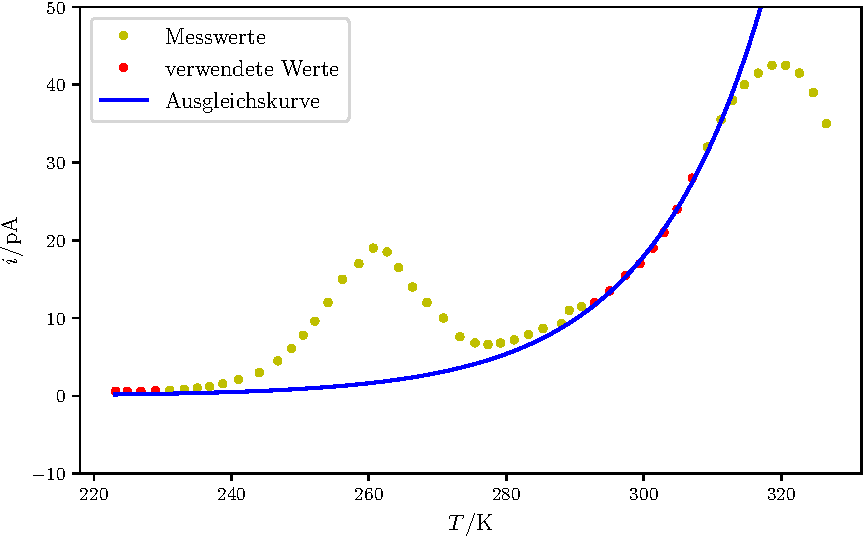
\includegraphics[width=\linewidth-60pt,height=\textheight-60pt,keepaspectratio]{content/images/plot1exp.pdf}
	\caption{Die Messdaten mit der Ausgleichskurve für die ansteigende Flanke des zweiten Peaks.}
	\label{fig:plot1exp}
\end{figure}

\begin{figure}
	\centering
	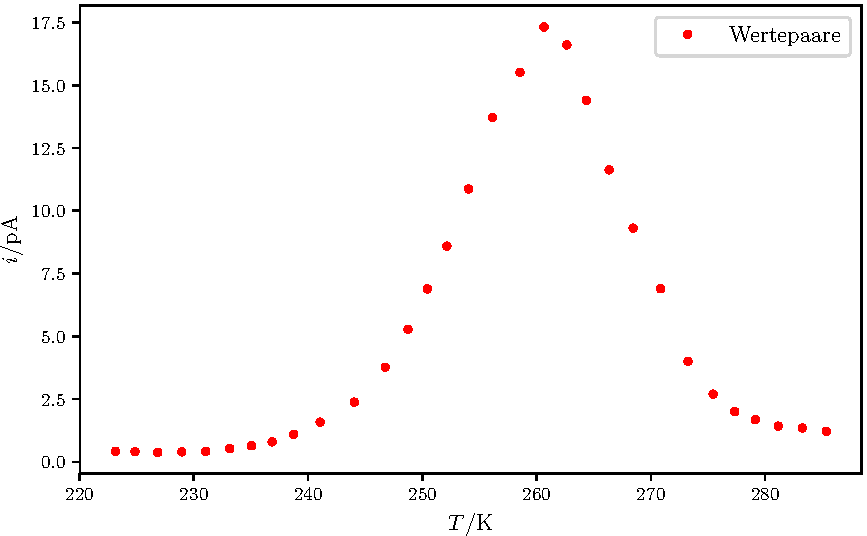
\includegraphics[width=\linewidth-60pt,height=\textheight-60pt,keepaspectratio]{content/images/bereinigt1.pdf}
	\caption{Die bereinigten Messdaten.}
	\label{fig:bereinigt1}
\end{figure}

\begin{figure}
	\centering
	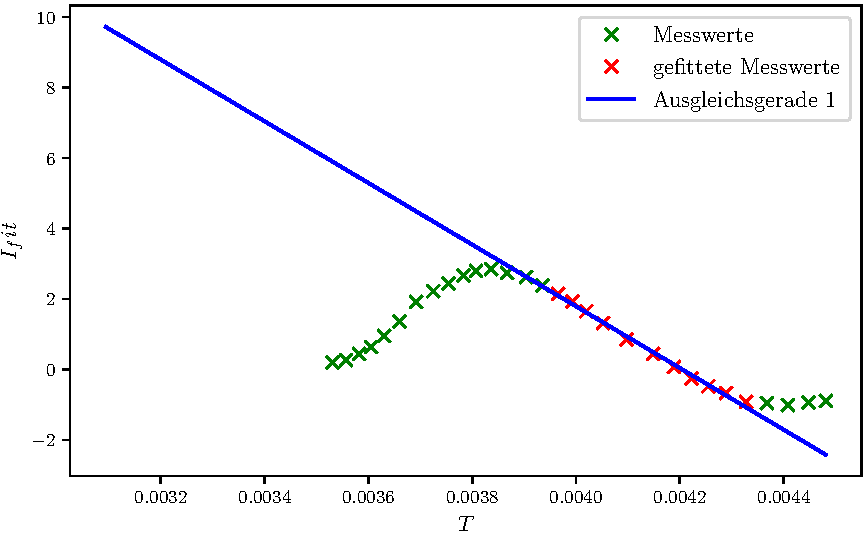
\includegraphics[width=\linewidth-60pt,height=\textheight-60pt,keepaspectratio]{content/images/W1_1.pdf}
	\caption{Die logarithmischen Werte gemäß Formel \eqref{eq:} aufgetragen gegen das Inverse der Temperatur.}
	\label{fig:W1_1}
\end{figure}

\begin{figure}
	\centering
	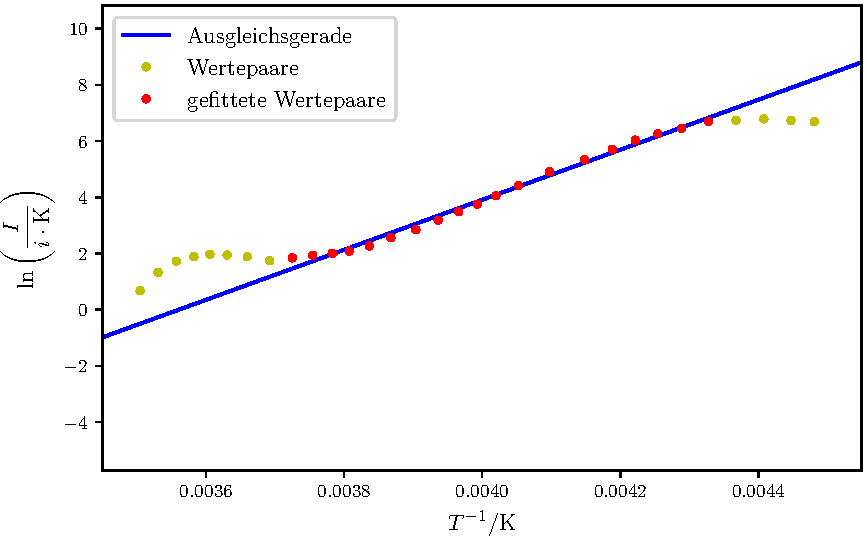
\includegraphics[width=\linewidth-60pt,height=\textheight-60pt,keepaspectratio]{content/images/W1_2.pdf}
	\caption{Die logarithmischen Werte gemäß Formel \eqref{eq:} aufgetragen gegen das Inverse der Temperatur.}
	\label{fig:W1_2}
\end{figure}

%\begin{table}
%	\centering
%	\caption{Die bereinigten, als auch die nicht bereinigten Messdaten, sowie die logarithmischen Werte gemäß Formel \eqref{eq:} und \eqref{eq:}.}
%	\label{tab:data1}
	\sisetup{table-format=1.2}
	\begin{tabular}{S[table-format=1.2]S[table-format=4.0]}
		\toprule
		{$\frac{\Delta s}{\si{\milli\meter}}$} & {$N$} \\
		\midrule
		5.00 & 3144 \\
		5.00 & 3105 \\
		5.00 & 3076 \\
		5.00 & 2973 \\
		5.00 & 3183 \\
		\bottomrule
	\end{tabular}

%	\label{tab:data1}
%\end{table}

\subsection{Bestimmung der Aktivierungsenergie $W$ und der charakteristischen Relaxatioszeit $\tau_.0$ bei einer Heizrate von $b=\SI{1,4}{\kelvin\per\minute}$}

Die erhobenen Messwerte des Polarisationsstroms werden mittels einer Regression der Form \eqref{eq:reg1} bereinigt. In Abbildung \ref{fig:plot2exp} sind die Rohdaten, die für den Fit verwendeten Werte, sowie der Fit selbst zu sehen.\\
Für die Parameter ergibt sich:
\begin{align*}
a_2&=\SI{6,24(14)e-2}{\pico\ampere}\\
b_2&=\SI{255,5(11)}{\kelvin}\text{.}\\
\end{align*}
In Abbildung \ref{fig:bereinigt2} sind die bereinigten Messwerte aufgetragen und in Tabelle \ref{tab:data2} gemeinsam mit den Rohdaten zu sehen.
Für kleine Temperaturen $T$ wird in Abbildung \ref{fig:W2_1} nach Gleichung \eqref{eq:ln1} das Logarithmierte des Polarisationsstrom $i$ gegen das Inverse der Temperatur aufgetragen. Die logarithmischen Werte sind ebenfalls in Tabelle \ref{tab:data2} eingetragen.
Die lineare Regression der Form \eqref{eq:reg2} liefert die Parameter:
\begin{align*}
\alpha_2&=\SI{}{\kelvin},\\
\beta_2 &= \text{.}
\end{align*}
Daraus lässt sich die Aktivierungsenergie $W$ berechnen zu:
\[
W_{2,1} = -\alpha_2 k_.B =\SI{1,145(15)e-19}{\joule}=\SI{0.714(8)}{\electronvolt}\text{.}
\]
Die Aktivierungsenergie lässt sich ebenfalls über den gesamten Kurvenverlauf bestimmen. Dazu wird nach Formel \eqref{eq:} eine Ausgleichsrechnung der Form \eqref{eq:reg3} durchgeführt. Dabei ist $T^*=\SI{}{}$. Es ergeben sich die Parameter:
\begin{align*}
m_2&=\SI{}{\kelvin},\\
n_2&=\SI{}{}\text{.}
\end{align*}
Der Graph ist in Abbildung \ref{fig:W2_2} zu sehen und die zugehörigen Werte in Tabelle \ref{tab:data2}.
Daraus ergibt sich $W$ zu:
\[
W_{2,2} = m_2 k_.B =\SI{1,237(14)e-19}{\joule}=\SI{0.772(9)}{\electronvolt}\text{.}
\]

\begin{figure}
	\centering
	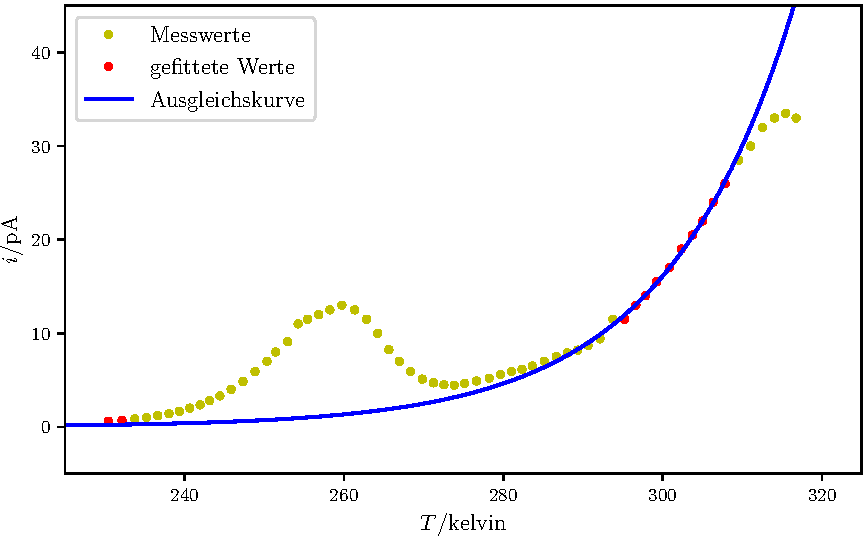
\includegraphics[width=\linewidth-60pt,height=\textheight-60pt,keepaspectratio]{content/images/plot2exp.pdf}
	\caption{Die Messdaten mit der Ausgleichskurve für die ansteigende Flanke des zweiten Peaks.}
	\label{fig:plot2exp}
\end{figure}

\begin{figure}
	\centering
	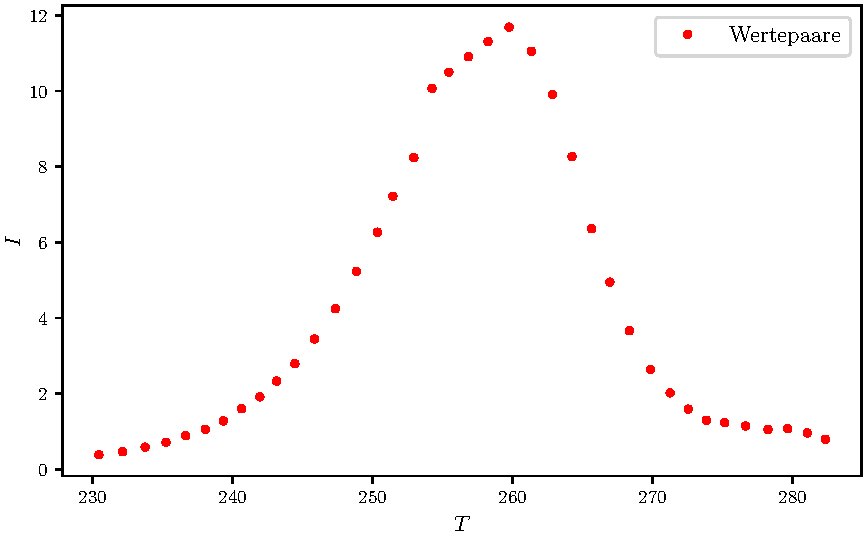
\includegraphics[width=\linewidth-60pt,height=\textheight-60pt,keepaspectratio]{content/images/bereinigt2.pdf}
	\caption{Die bereinigten Messdaten.}
	\label{fig:bereinigt2}
\end{figure}

\begin{figure}
	\centering
	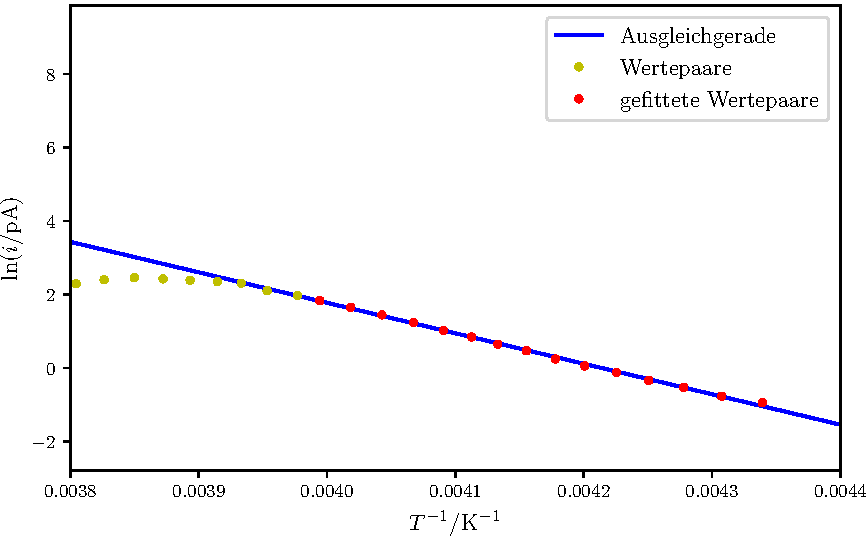
\includegraphics[width=\linewidth-60pt,height=\textheight-60pt,keepaspectratio]{content/images/W2_1.pdf}
	\caption{Die logarithmischen Werte gemäß Formel \eqref{eq:} aufgetragen gegen das Inverse der Temperatur.}
	\label{fig:W2_1}
\end{figure}

\begin{figure}
	\centering
	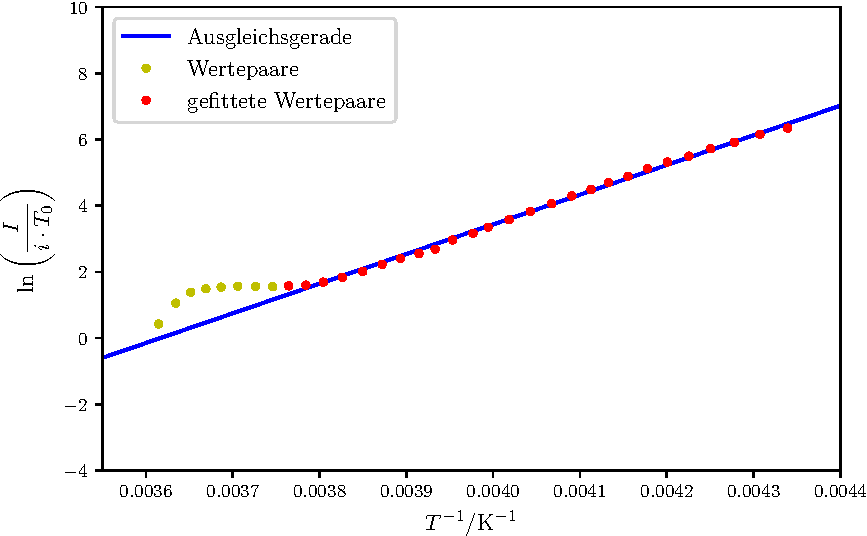
\includegraphics[width=\linewidth-60pt,height=\textheight-60pt,keepaspectratio]{content/images/W2_2.pdf}
	\caption{Die logarithmischen Werte gemäß Formel \eqref{eq:} aufgetragen gegen das Inverse der Temperatur.}
	\label{fig:W2_2}
\end{figure}

%\begin{table}
%	\centering
%	\caption{Die bereinigten, als auch die nicht bereinigten Messdaten, sowie die logarithmischen Werte gemäß Formel \eqref{eq:} und \eqref{eq:}.}
%	\label{tab:data2}
	\sisetup{table-format=1.2}
	\begin{tabular}{S[table-format=1.2]S[table-format=2.0]}
		\toprule
		{$\frac{\Delta p}{\si{\bar}}$} & {$N$} \\
		\midrule
		0.80 & 39 \\
		0.80 & 30 \\
		0.80 & 33 \\
		0.80 & 33 \\
		0.80 & 33 \\
		0.80 & 34 \\
		0.80 & 33 \\
		0.80 & 33 \\
		\bottomrule
	\end{tabular}

%	\label{tab:data2}
%\end{table}